%=======================02-713 LaTeX template, following the 15-210 template==================
%
% You don't need to use LaTeX or this template, but you must turn your homework in as
% a typeset PDF somehow.
%
% How to use:
%    1. Update your information in section "A" below
%    2. Write your answers in section "B" below. Precede answers for all 
%       parts of a question with the command "\question{n}{desc}" where n is
%       the question number and "desc" is a short, one-line description of 
%       the problem. There is no need to restate the problem.
%    3. If a question has multiple parts, precede the answer to part x with the
%       command "\part{x}".
%    4. If a problem asks you to design an algorithm, use the commands
%       \algorithm, \correctness, \runtime to precede your discussion of the 
%       description of the algorithm, its correctness, and its running time, respectively.
%    5. You can include graphics by using the command \includegraphics{FILENAME}
%
\documentclass[11pt]{article}
\usepackage{amsmath,amssymb,amsthm}
\usepackage{graphicx}
\usepackage[margin=1in]{geometry}
\usepackage{fancyhdr}
\usepackage{cancel}
\usepackage{mathtools}
\usepackage{tikz}
\DeclarePairedDelimiter{\ceil}{\lceil}{\rceil}

\setlength{\parindent}{0pt}
\setlength{\parskip}{5pt plus 1pt}
\setlength{\headheight}{13.6pt}
\newcommand\question[2]{\vspace{.25in}\hrule\textbf{#1: #2}\vspace{.5em}\hrule\vspace{.10in}}
\renewcommand\part[1]{\vspace{.10in}\textbf{(#1)}}
\newcommand\algorithm{\vspace{.10in}\textbf{Algorithm: }}
\newcommand\correctness{\vspace{.10in}\textbf{Correctness: }}
\newcommand\runtime{\vspace{.10in}\textbf{Running time: }}
\pagestyle{fancyplain}
\lhead{\textbf{\NAME\ (\ANDREWID)}}
\chead{\textbf{HW\HWNUM}}
\rhead{02-713, \today}
\begin{document}\raggedright
%Section A==============Change the values below to match your information==================
\newcommand\NAME{Carl Kingsford}  % your name
\newcommand\ANDREWID{ckingsf}     % your andrew id
\newcommand\HWNUM{1}              % the homework number
%Section B==============Put your answers to the questions below here=======================

% no need to restate the problem --- the graders know which problem is which,
% but replacing "The First Problem" with a short phrase will help you remember
% which problem this is when you read over your homeworks to study.
\newcommand{\sumn}{\sum_{n=0}^{\infty}}
\newcommand{\ea}{e^{\alpha}}
\newcommand{\nea}{e^{-\alpha}}
\newcommand{\solution}{\textbf{Solution: }\\}
\newcommand{\set}[1]{\{#1\}}
\newcommand{\N}{\mathbb{N}}
\newcommand{\Z}{\mathbb{Z}}
\newcommand{\R}{\mathbb{R}}

\question{Problem 1}{}
(a) Rewrite the following logical statement using only $\lnot$ and $\to$:
\[P \lor (R\land \lnot Q) \to (W \to Q)\]
\solution
\begin{align*}
    P \lor (R\land \lnot Q) \to (W \to Q) &\equiv \lnot(\lnot P) \lor (R\land \lnot Q) \to (W \to Q)\\
                                          &\equiv \lnot P \to (R \land \lnot Q) \to (W \to Q)\\
                                          &\equiv \lnot P \to \lnot(\lnot R \lor Q) \to (W \to Q)\\
                                          &\equiv \lnot P \to \lnot(R\to Q) \to (W \to Q)\\
\end{align*}

(b) Determine if the following is a tautology:
\[\lnot (P\lor (Q\land (\lnot R)))\longleftrightarrow (\lnot P) \land ((\lnot Q)\lor R)\]
\solution

In order to determine if the statement is a tautology, we can construct a truth table and see if the statement is true for all possible combinations of $P$, $Q$, and $R$.
\[
\begin{array}{|c|c|c|c|c|c|c|c|c|c|c|}
\hline
P & Q & R & \lnot (P \lor (Q \land (\lnot R))) & (\lnot P) \land ((\lnot Q) \lor R) \\
\hline
T & T & T & F & F \\
T & T & F & F & F \\
T & F & T & F & F \\
T & F & F & F & F \\
F & T & T & F & F \\
F & T & F & F & F \\
F & F & T & T & T \\
F & F & F & T & T \\
\hline
\end{array}
\]

Please note that "T" represents True and "F" represents False.
Thus, the statement is not a tautology.

(c) Which of these statements is true? Explain your answer.
\begin{itemize}
    \item If the world is flat, then $2+2=4$.
    \item If the above statement is true, then $2+2=5$.
\end{itemize}

\solution
The first statement is true. Since the world is not flat, the statement is vacuously true. The second statement is false because $2+2=5$ is false, and the first statement is true.

\question{Problem 2}{}
Let $C(x,y)$ denote the predicate that person $x$ is in class $y$.
\begin{itemize}
    \item Translate the following into English:\[\forall x\exists yC(x, y)\]\[\forall y\exists xC(x, y)\]
    \item Are the above statements equivalent? Does one imply the other? Justify your answers.
\end{itemize}
\solution

The first statement translates to "For all people, there exists a class that they are in." The second statement translates to "For all classes, there exists a person that is in that class."

They are not equivalent. Assume that there are $3$ people and $3$ classes. All people attend class $A$, so in this case the first statement is true.
Now if no person attend class B, then the second statement is false. Thus, the statements are not equivalent.

(b) Negate the following statement and simplify: your solution should have \textbf{no} $\lnot$.

\[\forall x\in \mathbb{R}(x < 0 \to \exists q\in \mathbb{R}(x < q \land q < 0))\]

\solution
\begin{align*}
    &\lnot \forall x\in \mathbb{R}(x < 0 \to \exists q\in \mathbb{R}(x < q \land q < 0))\\
    &\equiv \exists x\in \mathbb{R} \lnot (x < 0 \to \exists q\in \mathbb{R}(x < q \land q < 0))\\
    &\equiv \exists x\in \mathbb{R} \lnot (\lnot (x < 0) \lor \exists q\in \mathbb{R}(x<q\land q < 0))\\
    &\equiv \exists x\in\mathbb{R} (x < 0) \land (\lnot\exists q\in \mathbb{R}(x<q\land q < 0)) \\
    &\equiv \exists x\in\mathbb{R} (x < 0) \land (\forall q\in \mathbb{R}\lnot(x<q\land q < 0)) \\
    &\equiv \exists x\in\mathbb{R} (x < 0) \land (\forall q\in \mathbb{R}(x\geq q\lor q \geq 0)) \\
\end{align*}
(c) Write the following statements in predicate logic:
\begin{itemize}
    \item If there is a printer that loses all print jobs, then not everything will be printed.
    \item If no print jobs are lost by any printers, then everything will be printed
\end{itemize}
\solution
\begin{itemize}
    \item $\exists x\in \text{Printers}(\forall y\in \text{PrintJobs}(Loses(x,y)) \to \lnot \forall z\in \text{PrintJobs}(Printed(z)))$
    \item $\lnot \exists x\in \text{Printers}(\forall y\in \text{PrintJobs}(\lnot Loses(x,y)) \to \lnot \forall z\in \text{PrintJobs}(Printed(z)))$
\end{itemize}

(d) Assume P is a set, and Sick($x$) is the predicate that person $x$ is sick. Are the following statements true if there is at least one sick person in $P$ and at least one not sick person in $P$?
\begin{itemize}
    \item $(\forall x\in P, Sick(x))\to (\exists y\in P, Sick(y))$
    \item $\forall x\in P, (Sick(x)\to (\exists y\in P, Sick(y)))$
\end{itemize}

\solution

Both statements are true. The first statement can be rewritten as
\[\lnot (\forall x\in P, Sick(x)) \lor (\exists y\in P, Sick(y))\]
Since there is at least one sick person in $P$, the first statement is true.

The second statement can be rewritten as
\[\forall x\in P, \lnot Sick(x) \lor (\exists y\in P, Sick(y))\]
Since there is at least one sick person in $P$, the second statement is true.

(e) Suppose that $A,B,C$ are sets and $A\in B$, $B\subseteq C$. Is it true that $A\subseteq C$?
\solution

No. Consider the following example:
\begin{align*}
    A &= \{1,2\}\\
    B &= \{\{1,2\}, \{1\}\}\\
    C &= \{\{1,2\}, \{1\}, 3\}
\end{align*}
We have $A\in C$ but $A\not\subseteq C$.

(f) Are the following sets the same? $P(\set{1,2,3})\cup P(\set{4})$ and $P(\set{1,2,3,4})$
\solution

No. Since $\set{1,2,3,4}\in P(\set{1,2,3,4})$ and $\set{1,2,3,4}\not\in P(\set{1,2,3})\cup P(\set{4})$, the two sets are not the same.

\question{Problem 3}{}

Decide if the following functions are surjective or injective or bijective or not defined.

\begin{itemize}
    \item $f: \N\to\Z, f(n)=n^2-|n|$
    \item $f: \Z\to\N, f(n)=|n|-6$
    \item $f: \R\to\R^{+}, f(x) = \sqrt{x} +6$
    \item $f:P(\N)\to \N, f(B)=|B\cup \set{3,4,5,\cdots, 10}|$
\end{itemize}

\solution

% make an array to check if each function is surjective, injective, bijective, well-defined
\[
\begin{array}{|c|c|c|c|c|}
\hline
\text{Function} & \text{Surjective} & \text{Injective} & \text{Bijective} & \text{well-defined} \\
\hline
f: \N\to\Z, f(n)=n^2-|n| & \text{No} & \text{No} & \text{No} & \text{Yes} \\
f: \Z\to\N, f(n)=|n|-6 & \text{Yes} & \text{No} & \text{No} & \text{Yes} \\
f: \R\to\R^{+}, f(x) = \sqrt{x} +6 & \text{No} & \text{Yes} & \text{No} & \text{No} \\
f:P(\N)\to \N, f(B)=|B\cup \set{3,4,5,\cdots, 10}| & \text{No} & \text{No} & \text{No} & \text{Yes}\\
\hline
\end{array}
\]

(b) Supose that $A \subset B$ (which means $A$ is a subset of $B$, but $A \neq B$). Give an example of a surjective function $f : A \to B$.

\solution

Let $B = \N$, and $A = 2\N$(even numbers), and $f(x) = x/2$. Then $f$ is surjective.
This is because for any $y\in \N$, we can find $x = 2y\in 2\N$ such that $f(x) = 2y/2 = y$.

(c) Let $f:\Z\to \Z, f(x) = x^2 + 5$ show that $f$ is not injective, and find $f^{-1}(\set{x|x>10})$

\solution

$f$ is not injective because $f(2) = f(-2) = 9$. for $x \ge 3$, $f(x) > 10$, so $f^{-1}(\set{x|x>10}) = \set{x|x\ge 3}$.

\qed

(d) Let $A = \set{x\in \R|-5 < x < 5}$, For each of the following sets, determine if it has the same cardinality as $A$:
\begin{itemize}
    \item $\set{x\in \R|0 \leq x \leq 1}$
    \item $\set{x\in \N | -5 \le x\le 5}$
\end{itemize}

\solution

The first set has the same cardinality as $A$ because we can construct a bijection between the two sets. Let $f(x) = 5x-5$, then $f$ is a bijection between the two sets.

The second set does not have the same cardinality as $A$ because there is no bijection between the two sets, since the cardinality of the second set is $6$, while $A$ is infinite. 

\question{Problem 4: Growth of Function}{}

Find a big-Oh notation for the function (proving your result using the definitions from
class). 

\[(2^n + n ^2)(n+n(\log_2{n}))\]

\solution

For sufficiently large $n$, we have

\begin{align*}
    (2^n + n ^2)(n+n(\log_2{n})) &= n^3 + n^3\log_2{n} + 2^n + 2^n\log_2{n}\\
                                 &\le 2n^3\log_2{n} + 2\cdot2^n\log_2{n}\\
                                 &\le 2\cdot2^{n}\log_2{n} + 2\cdot2^n\log_2{n}\\
                                 &\le 4\cdot2^{n}\log_2{n}\\
                                 &= O(2^n\log_2{n})
\end{align*}

(b) Answer the following using the definitions from class:
\begin{itemize}
    \item Is $f(n) = 2^{2n} O(2^n)$ ?
    \item Is $f(n) = n^2 O\left(n^{5/2}\right)$ ?
\end{itemize}

\solution

$f(n) = 2^{2n}$ is not $O(2^n)$ because
\[2^{2n} = 2^{n} \times 2^{n}\]
$2^n$ as $n$ $\to \infty$. Thus there is no constant $c$ such that $2^{2n} \le c2^n$ for all $n$.

$f(n) = n^2$ is $O\left(n^{5/2}\right)$ because for $n\ge 1$,
\[n^2 \le n^{2.5} \le n^{5/2}\]
Thus by definition of big-$O$, $f(n) = O\left(n^{5/2}\right)$.

\qed


(c) Show that $f(n) = (n+\log(n))(5n + \sqrt{n})$ is $\Theta(n^2)$.

\solution

For sufficiently large $n$, we have

\begin{align*}
    f(n) &= (n+\log(n))(5n + \sqrt{n})\\
         &= 5n^2 + n\sqrt{n} + 5n\log(n) + \sqrt{n}\log(n)\\
         &\le 5n^2 + n^2 + 5n^2 + n^2\\
         &= 12n^2\\
         &= O(n^2)
\end{align*}

also
\begin{align*}
    f(n) \ge n \cdot 5n = 5n^2 = \Omega(n^2)
\end{align*}

Thus, $f(n) = \Theta(n^2)$.

(d) For the following functions, decide if $f(n)$ is $O(g(n))$ or $f(n)$ is $\omega(g(n))$ or both. Prove your answer.
\begin{itemize}
    \item $f(n) = \sqrt{n}, g(n) = \log(n)^2$
    \item $f(n) = (3^n +\log(n))(n^2 +2^n\log(n)), g(n)=4^n$
\end{itemize}

\solution

For large $n$
\begin{align*}
    f(n) &= \sqrt{n}\\
         &= n^{1/4}n^{1/4}\\
         &\ge \log(n^{1/4})\log(n^{1/4})\\
         &= \log(n^{1/4})^2 = \frac{1}{16} \log(n)^2\\
         &= \Omega(\log(n)^2)
\end{align*}

Thus, $f(n) = \Omega(g(n))$.

For the second function, we have

\begin{align*}
    f(n) &= (3^n +\log(n))(n^2 +2^n\log(n))\\
         &= 6^n\log(n) + n^2\log(n) + 3^nn^2 + 2^n\log^2(n)\\
         &\ge 6^n > 4^n
\end{align*}

Thus, $f(n) = \Omega(g(n))$.

\question{Problem 5: Sequences, Summations}{}

(a) Find the sum if it exists:
\begin{equation}
    \frac{1}{3} + \frac{2}{9} + \frac{4}{27} + \frac{8}{81} + \cdots
\end{equation}

\solution

Let $S$ be the sum of the series. Then we have
\begin{align*}
    S &= \sum_{n=0}^{\infty}\frac{2^n}{3^{n+1}}\\
      &= \frac{1}{3}\sum_{n=0}^{\infty}\frac{2^n}{3^n}\\
      &= \frac{1}{3}\sum_{n=0}^{\infty}\left(\frac{2}{3}\right)^n\\
      &= \frac{1}{3}\frac{1}{1-2/3} = 1
\end{align*}

(b) Find the sum if it exists:
\begin{equation}
    \sum_{n=1}^{\infty} 2(-1)^{\ceil{\frac{n}{2}}}
\end{equation}

\solution

$n$ can be classified according to mod $4$. We have
\[n = 4k, 4k+1, 4k+2, 4k+3\]


Let $S_{n}$ be the sum of the series. Then we have
\begin{align*}
    S_{4N} &= \sum_{n=1}^{4N} 2(-1)^{\ceil{\frac{n}{2}}}\\
      &= \sum_{k=0}^{N} \left(2(-1)^{\ceil{\frac{4k}{2}}} + 2(-1)^{\ceil{\frac{4k+1}{2}}} + 2(-1)^{\ceil{\frac{4k+2}{2}}} + 2(-1)^{\ceil{\frac{4k+3}{2}}}\right)\\
      &= \sum_{k=0}^{N} \left(2(-1)^{2k} + 2(-1)^{2k+1} + 2(-1)^{2k+1} + 2(-1)^{2k+2}\right)\\
      &= \sum_{k=0}^{N} \left(2 - 2 - 2 + 2\right) = 0\\
\end{align*}

\begin{align*}
    S_{4N+1} &= \sum_{n=1}^{4N+1} 2(-1)^{\ceil{\frac{n}{2}}}\\
      &= 2(-1)^{\ceil{(4N+1)/2}} + \sum_{k=0}^{N} \left(2(-1)^{\ceil{\frac{4k}{2}}} + 2(-1)^{\ceil{\frac{4k+1}{2}}} + 2(-1)^{\ceil{\frac{4k+2}{2}}} + 2(-1)^{\ceil{\frac{4k+3}{2}}}\right)\\
      &= 2 + \sum_{k=0}^{N} \left(2(-1)^{2k+1} + 2(-1)^{2k+1} + 2(-1)^{2k+2} + 2(-1)^{2k+2}\right)\\
      &= 2 + \sum_{k=0}^{N} \left(-2 - 2 + 2 + 2\right) = 2\\
\end{align*}

Therefore, the sum does not converge, since $S_{4N}$ and $S_{4N+1}$ do not converge. This implies that the sum does not exist.

\qed

(c)  Find the sum (using a formula from class):
\begin{equation}
    \sum_{i=3}^{\infty} \left(\frac{1}{3}\right)^i
\end{equation}

\solution

\begin{align*}
    \sum_{i=3}^{\infty} \left(\frac{1}{3}\right)^i
    &= \sum_{k=0}^{\infty} \frac{1}{9}\left(\frac{1}{3}\right)^k\\
    &= \frac{1}{9}\sum_{k=0}^{\infty} \left(\frac{1}{3}\right)^k\\
    &= \frac{1}{9}\frac{1}{1-1/3} = \frac{1}{6}
\end{align*}

\qed

\question{Problem 6}{Binary Relations}

(a) Let $X = \set{1,2,3}$, Let $R$ be a binary relation over the power set $P(X)$, defined in the following way: for $A, B\in P(X)$, we have $(A, B)\in R$ iff $A\subseteq B$ and $|B-A|\le 1$.
Draw a graph that represents this binary relation. Determine which of the following properties the relation has:
\begin{itemize}
    \item Reflexive
    \item Symmetric
    \item Antisymmetric
    \item Transitive
\end{itemize}
Prove your answers.

\solution

The graph is shown below:

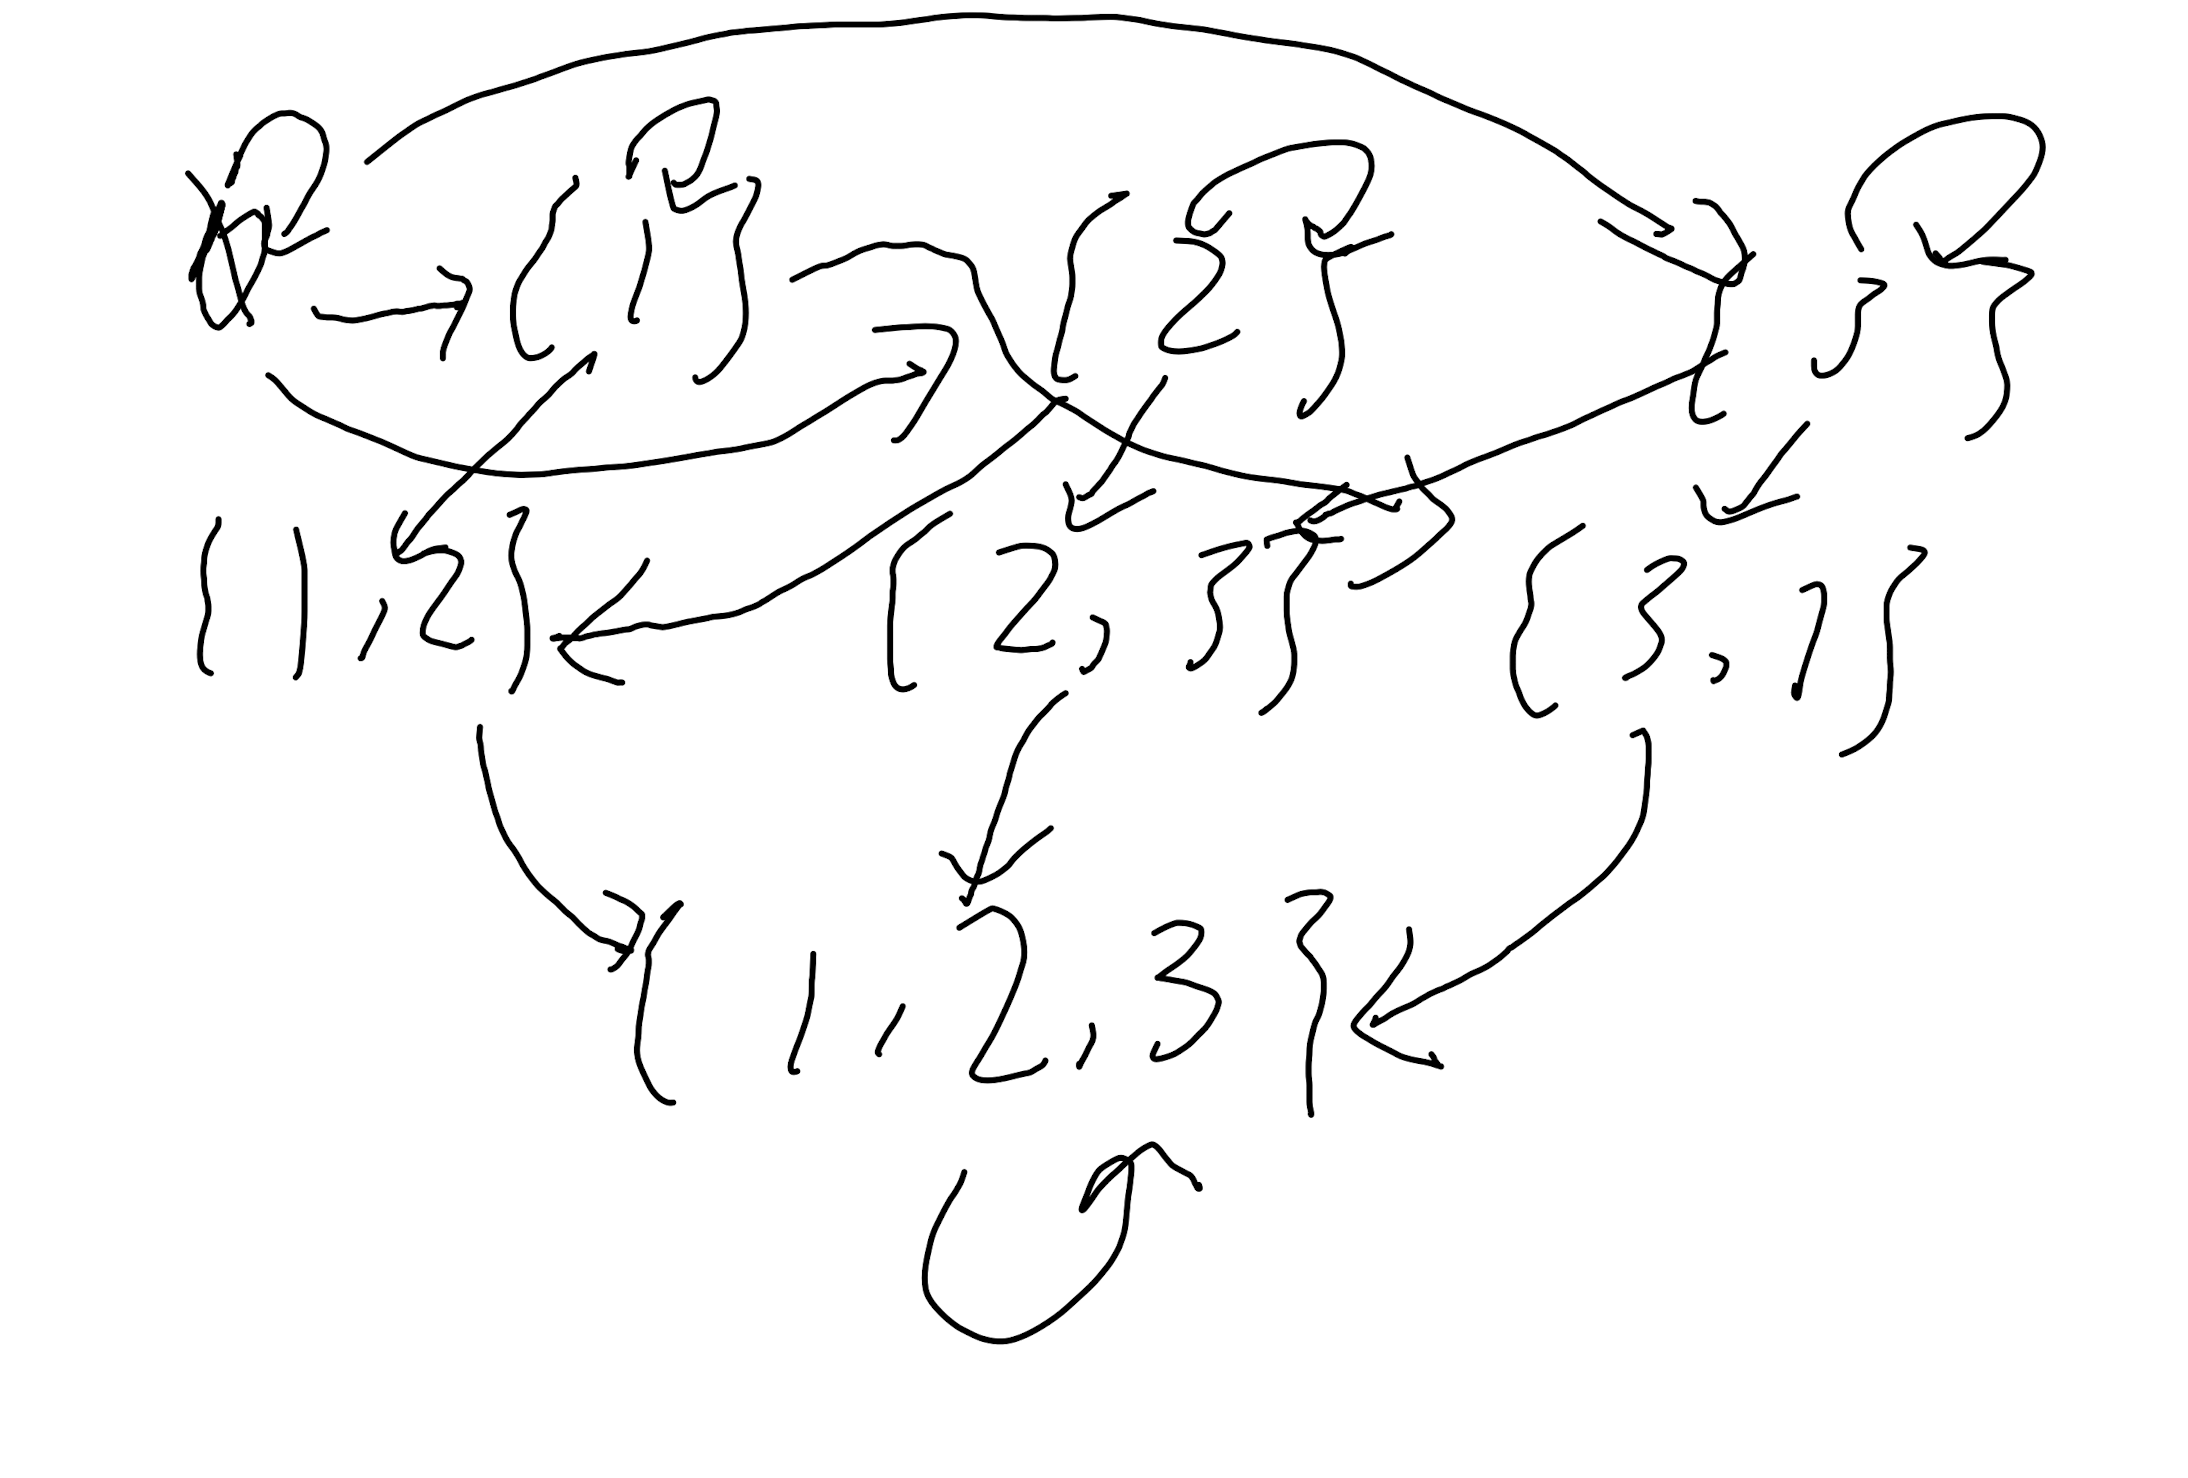
\includegraphics[width=10cm]{6a.png}

\begin{itemize}
    \item Reflexive: A binary relation $R$ is reflexive if every element is related to itself. In this case, for every $A \in P(X)$, we can see that $(A, A) \in R$ because $A \subseteq A$ and $|A - A| = 0 \le 1$. Therefore, $R$ is reflexive.
    \item Symmetric: A binary relation $R$ is symmetric if whenever $(A, B) \in R$, then $(B, A) \in R$. Looking at the directed graph, we can see that not all edges have a corresponding reverse edge. For example, there is an edge from $\emptyset$ to ${1}$, but there is no edge from ${1}$ to $\emptyset$. Hence, $R$ is not symmetric.
    \item Antisymmetric: A binary relation $R$ is antisymmetric if whenever $(A, B) \in R$ and $(B, A) \in R$, then $A = B$. By observing the directed graph, we can see that there are no pairs of distinct vertices with edges in both directions. Therefore, there are no two distinct elements $A$ and $B$ such that $(A, B) \in R$ and $(B, A) \in R$. Thus, $R$ is vacuously antisymmetric.
    \item For a relation to be transitive, if $(A, B) \in R$ and $(B, C) \in R$, then it should follow that $(A, C) \in R$. Let's consider an example to demonstrate that $R$ is not transitive. Take $A = \emptyset$, $B = \set{1}$, and $C = \set{1, 2}$. We can see that $(A, B) \in R$ because $A \subseteq B$ and $|B - A| = 1$. Similarly, $(B, C) \in R$ because $B \subseteq C$ and $|C - B| = 1$. However, $(A, C) \notin R$ because $A \nsubseteq C$.Therefore, since we can find specific counterexamples where $(A, B) \in R$ and $(B, C) \in R$ but $(A, C) \notin R$, we can conclude that $R$ is not transitive.
\end{itemize}

(b) Draw the graph for the relation $R\circ R\circ R$ on the same set $P(X)$.

\solution

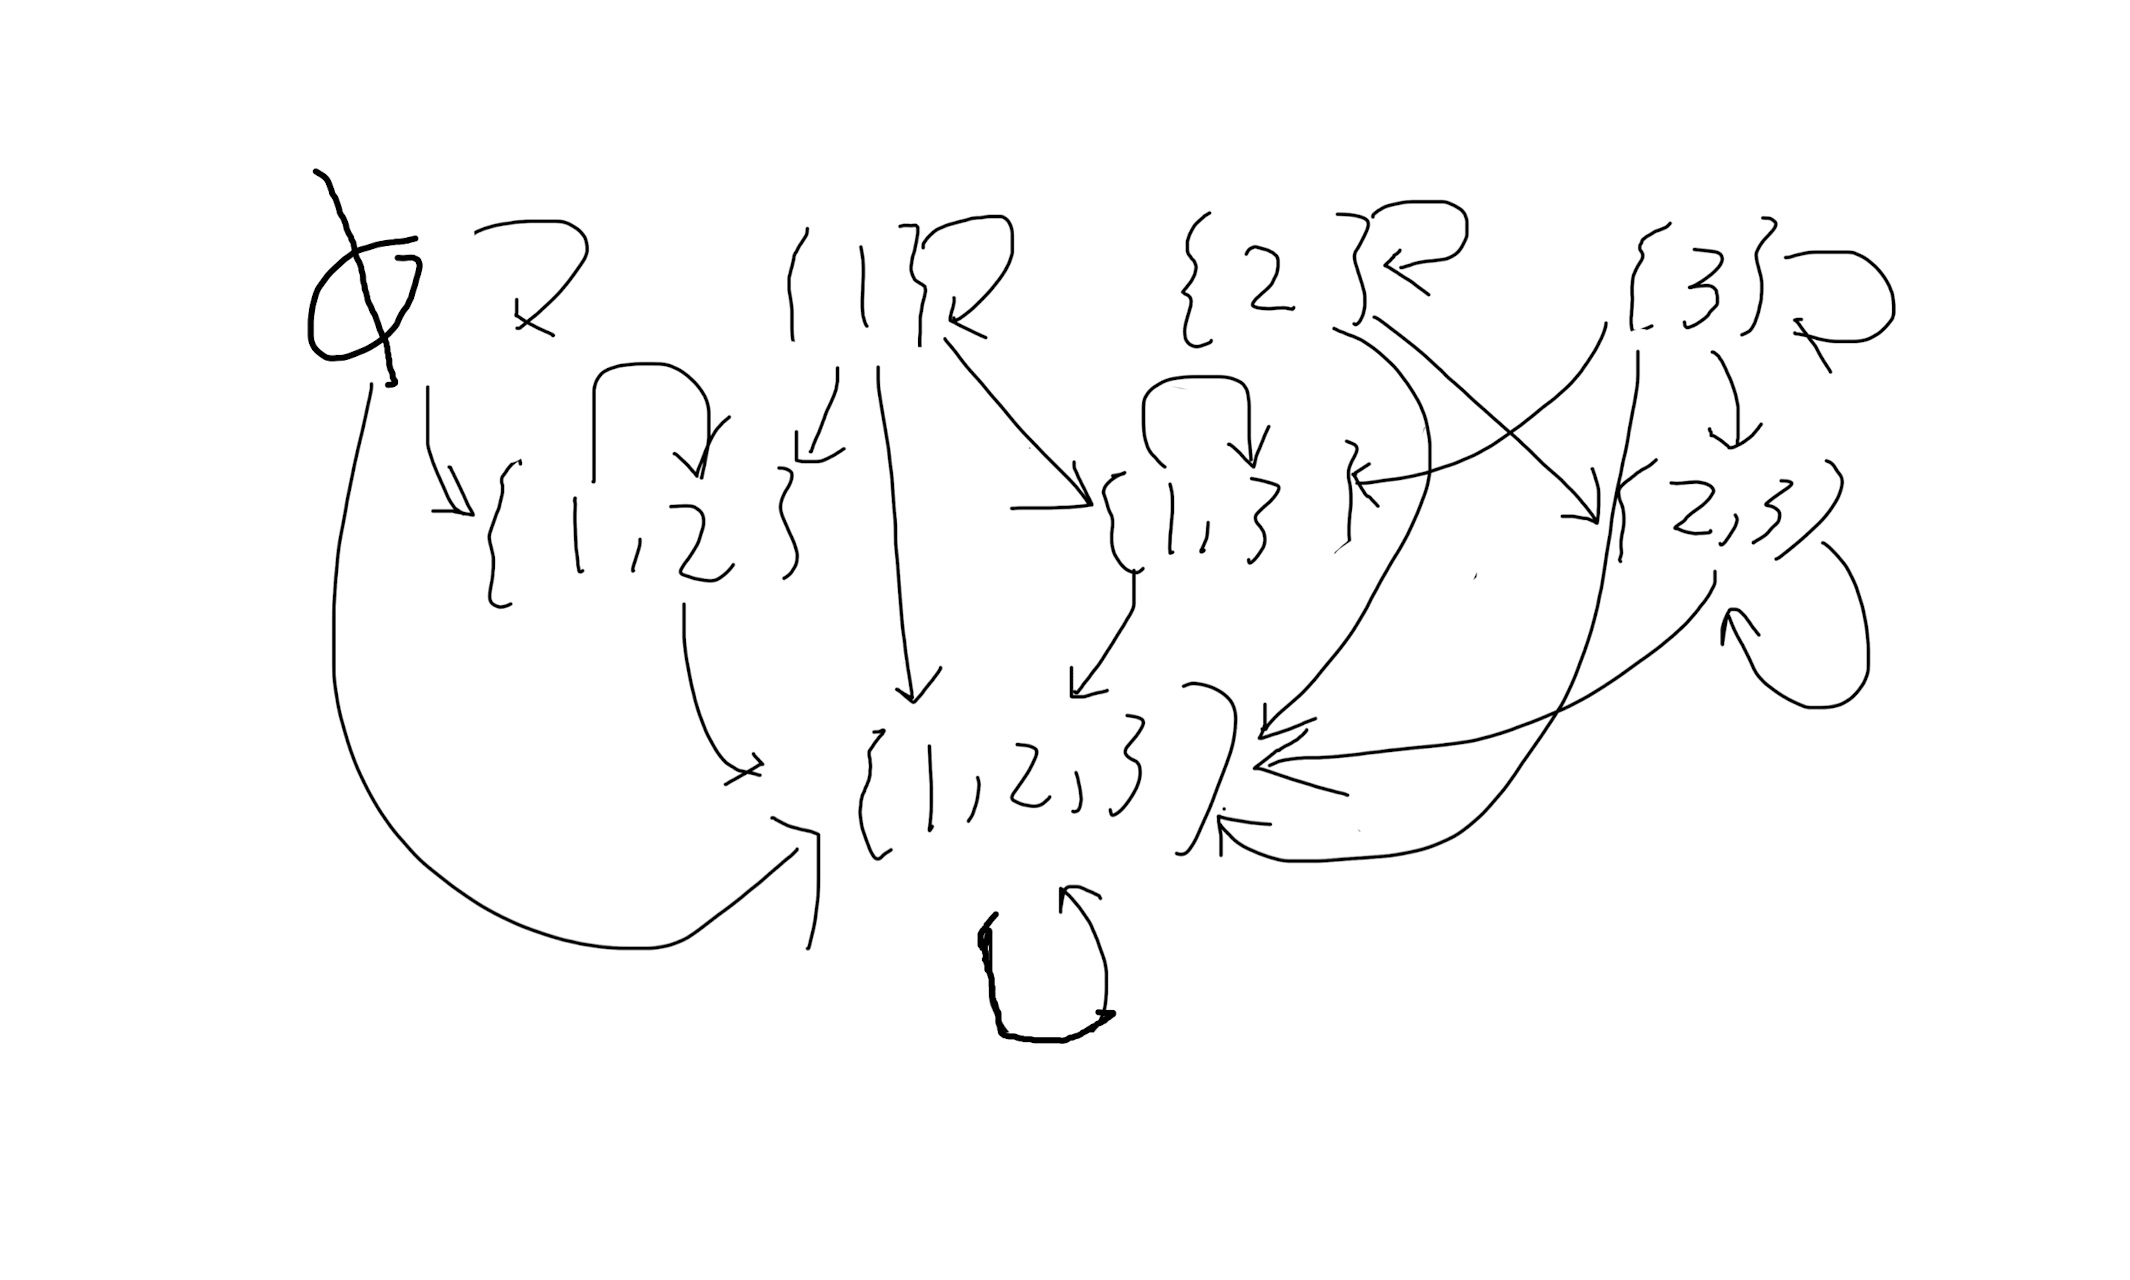
\includegraphics[width=10cm]{6b.png}

\end{document}